%%%%%%%%%%%%%%%%%%%%%%%%%%%%%%%%%%%%%%%%%
% Beamer Presentation
% LaTeX Template
% Version 1.0 (10/11/12)
%
% This template has been downloaded from:
% http://www.LaTeXTemplates.com
%
% License:
% CC BY-NC-SA 3.0 (http://creativecommons.org/licenses/by-nc-sa/3.0/)
%
%%%%%%%%%%%%%%%%%%%%%%%%%%%%%%%%%%%%%%%%%

%----------------------------------------------------------------------------------------
%   PACKAGES AND THEMES
%----------------------------------------------------------------------------------------

\documentclass{beamer}

\mode<presentation> {

%dencoding
%--------------------------------------
\usepackage[utf8]{inputenc}
\usepackage[T1]{fontenc}
%--------------------------------------

%Portuguese-specific commands
%--------------------------------------
\usepackage[portuguese]{babel}
%--------------------------------------

%Hyphenation rules
%--------------------------------------
\usepackage{hyphenat}
\hyphenation{mate-mática recu-perar}
%--------------------------------------

%--------------------------------------
\usepackage{textpos}
%--------------------------------------


\bibliographystyle{plain}

% The Beamer class comes with a number of default slide themes
% which change the colors and layouts of slides. Below this is a list
% of all the themes, uncomment each in turn to see what they look like.

%\usetheme{default}
%\usetheme{AnnArbor}
%\usetheme{Antibes}
%\usetheme{Bergen}
%\usetheme{Berkeley}
%\usetheme{Berlin}
%\usetheme{Boadilla}
%\usetheme{CambridgeUS}
%\usetheme{Copenhagen}
%\usetheme{Darmstadt}
%\usetheme{Dresden}
%\usetheme{Frankfurt}
%\usetheme{Goettingen}
%\usetheme{Hannover}
%\usetheme{Ilmenau}
%\usetheme{JuanLesPins}
%\usetheme{Luebeck}
%\usetheme{Madrid}
\usetheme{Malmoe}
%\usetheme{Marburg}
%\usetheme{Montpellier}
%\usetheme{PaloAlto}
%\usetheme{Pittsburgh}
%\usetheme{Rochester}
%\usetheme{Singapore}
%\usetheme{Szeged}
%\usetheme{Warsaw}


% As well as themes, the Beamer class has a number of color themes
% for any slide theme. Uncomment each of these in turn to see how it
% changes the colors of your current slide theme.

%\usecolortheme{albatross}
%\usecolortheme{beaver}
%\usecolortheme{beetle}
%\usecolortheme{crane}
\usecolortheme{dolphin}
%\usecolortheme{dove}
%\usecolortheme{fly}
%\usecolortheme{lily}
%\usecolortheme{orchid}
%\usecolortheme{rose}
%\usecolortheme{seagull}
%\usecolortheme{seahorse}
%\usecolortheme{whale}
%\usecolortheme{wolverine}

%\setbeamertemplate{footline} % To remove the footer line in all slides uncomment this line
\setbeamertemplate{footline} % To replace the footer line in all slides with a simple slide count uncomment this line

\setbeamertemplate{footline}{
\leavevmode%
  \hbox{%
  \begin{beamercolorbox}[wd=.4\paperwidth,ht=2.25ex,dp=1ex,center]{author in head/foot}%
    \usebeamerfont{author in head/foot}\insertshortauthor
  \end{beamercolorbox}%
  \begin{beamercolorbox}[wd=.6\paperwidth,ht=2.25ex,dp=1ex,center]{title in head/foot}%
    \usebeamerfont{title in head/foot}\insertshorttitle\hspace*{6em}
    \insertframenumber{} / \inserttotalframenumber\hspace*{1ex}
  \end{beamercolorbox}}%
  \vskip0pt
}

\setbeamertemplate{navigation symbols}{} % To remove the navigation symbols from the bottom of all slides uncomment this line
}

\usepackage{graphicx} % Allows including images
\usepackage{booktabs} % Allows the use of \toprule, \midrule and \bottomrule in tables

\addtobeamertemplate{frametitle}{}{%
\begin{textblock*}{100mm}(-.09\textwidth,-1.75cm)

\includegraphics[height=.1\textwidth]{./imagens/coders.png}
\end{textblock*}
}
%%----------------------------------------------------------------------------------------
%   TITLE PAGE
%----------------------------------------------------------------------------------------
%square bracket
\newcommand{\lcol}{{[}}
\newcommand{\rcol}{{]}}
\newcommand{\lista}[1]{\lcol#1\rcol}

%cores
%--------------------------------------
\newcommand{\azul}[1]{\textcolor{blue}{#1}}

\newcommand{\vermelho}[1]{\textcolor{red}{#1}}

\newcommand{\verde}[1]{\textcolor{green}{#1}}

%--------------------------------------
\title[Expressões Regulares]{Expressões Regulares na Prática!} % The short title appears at the bottom of every slide, the full title is only on the title page

\author[Yudi Matsuzake]{Gustavo Yudi Bientinezi Matsuzake\\
			
\includegraphics[height=1cm,width=2cm]{./imagens/coders.png}} % Your name

\institute[UTFPR] % Your institution as it will appear on the bottom of every slide, may be shorthand to save space
{
Universidade Tecnológica Federal do Paraná\\ % Your institution for the title page
Coders UTFPR\\
\medskip
\textit{matsuzake@alunos.utfpr.edu.br} % Your email address
\url{https://github.com/yudi-matsuzake/regex-coders}
}
\date{\today} % Date, can be changed to a custom date

\begin{document}

\begin{frame}
\titlepage % Print the title page as the first slide
\end{frame}

\newcommand{\sumario}{
\begin{frame}[allowframebreaks]{Outline}
\frametitle{Sumário} % Table of contents slide, comment this block out to remove it
\tableofcontents % Throughout your presentation, if you choose to use \section{} and \subsection{} commands, these will automatically be printed on this slide as an overview of your presentation
\end{frame}
}

\sumario

%----------------------------------------------------------------------------------------
%   PRESENTATION SLIDES
%----------------------------------------------------------------------------------------

\section{Introdução} 
\frame{\tableofcontents[currentsection]}

\subsection{O que é?} % A subsection can be created just before a set of slides with a common theme to further break down your presentation into chunks

%-----------------------------------------------
\begin{frame}
	\frametitle{Definição}

	\Large{\azul{\textbf{Expressão Regular}} é:}

	\begin{itemize}
		\item Uma "linguagem de programação"\cite{hopcroft};
		\item Intimamente relacionada aos \azul{DFA}, que são \textit{\azul{autômatos}}, analisadores sintáticos\cite{hopcroft};
		\item Uma maneira sucinta e \azul{finita} de representar uma linguagem infinita - regular;
		\item É um método formal de se especificar um padrão de texto\cite{aurelio}.
	\end{itemize}

\end{frame}

%------------------------------------------------
\begin{frame}
	\begin{block}{Mesmo, Eu.}
	"Uma imagem vale mais do que mil palavras. Uma Expressão Regular\footnote{bombeável} vale infinitas."
	\end{block}
\end{frame}
%------------------------------------------------

\begin{frame}
	\frametitle{Observação importante:}
	\centering \Large{Diferença da teoria e da prática.}
\end{frame}

%------------------------------------------------
\subsection{Parte prática!}

\begin{frame}
	\Large{\azul{\textbf{Vamos deixar claro nosso escopo!}}}
\end{frame}

%------------------------------------------------
\begin{frame}
	\frametitle{Para a felicidade de alguns, infelicidade de outros...}
	
	\begin{itemize}
		\item Nosso escopo nessa apresentação é mais \azul{prático} e não teórico;
		\item Vamos aprender \azul{como} usar;
		\item Vamos aprender \azul{onde} usar;
		\item Vamos aprender \azul{porque} usar.
	\end{itemize}
\end{frame}

\subsection{Você não vai aprender isso nessa apresentação!}

%------------------------------------------------
\begin{frame}
\frametitle{Nada de lógica}
\centering
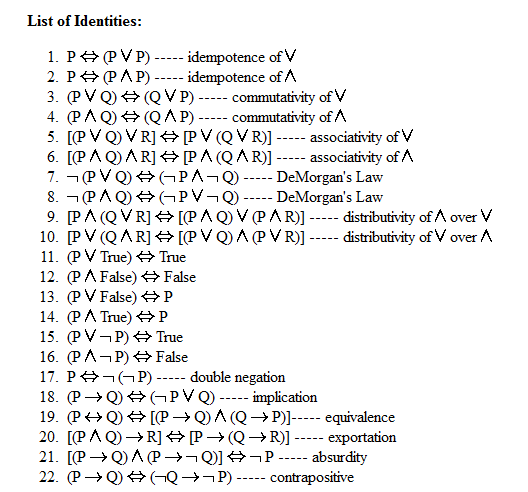
\includegraphics[width=0.8\textwidth]{./imagens/re/logica.png}
\end{frame}
%------------------------------------------------
\begin{frame}
\frametitle{Nada de transição de DFA para NFA}
\centering
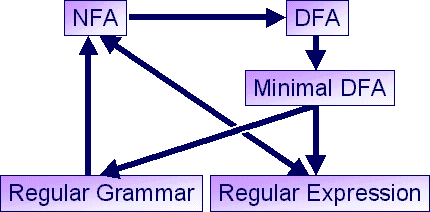
\includegraphics[width=0.8\textwidth]{./imagens/re/NFA-DFA.png}
\end{frame}
%------------------------------------------------
\begin{frame}
\frametitle{Não vamos aprender autômatos}
\centering
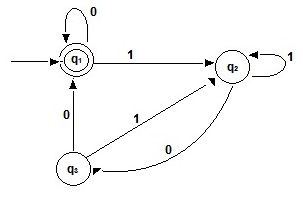
\includegraphics[width=0.8\textwidth]{./imagens/re/NFA.jpg}
\end{frame}
%------------------------------------------------

\subsection{Você vai aprender muito isso!}
%------------------------------------------------
\begin{frame}
\frametitle{Isso vai fazer parte da sua realidade}
\centering
\bf
\Large{\textasciicircum *[A-Za-z0-9\_]+:(.*)\$}
\end{frame}
%------------------------------------------------
\begin{frame}
\frametitle{Isso não vai te dar mais pânico!}
\centering
\bf
\Large{([0-9]\{1,3\}\textbackslash.)\{2\}[0-9]\{1,3\}-[0-9]\{2\}}
\end{frame}
%------------------------------------------------
\begin{frame}
\frametitle{Isso será fácil de entender (:}
\centering
\bf
\Large{[-+]?[0-9]\{1,3\}(\textbackslash.[0-9]\{3\})?(,[0-9]\{2\})?}
\end{frame}
%------------------------------------------------
\begin{frame}
\begin{figure}
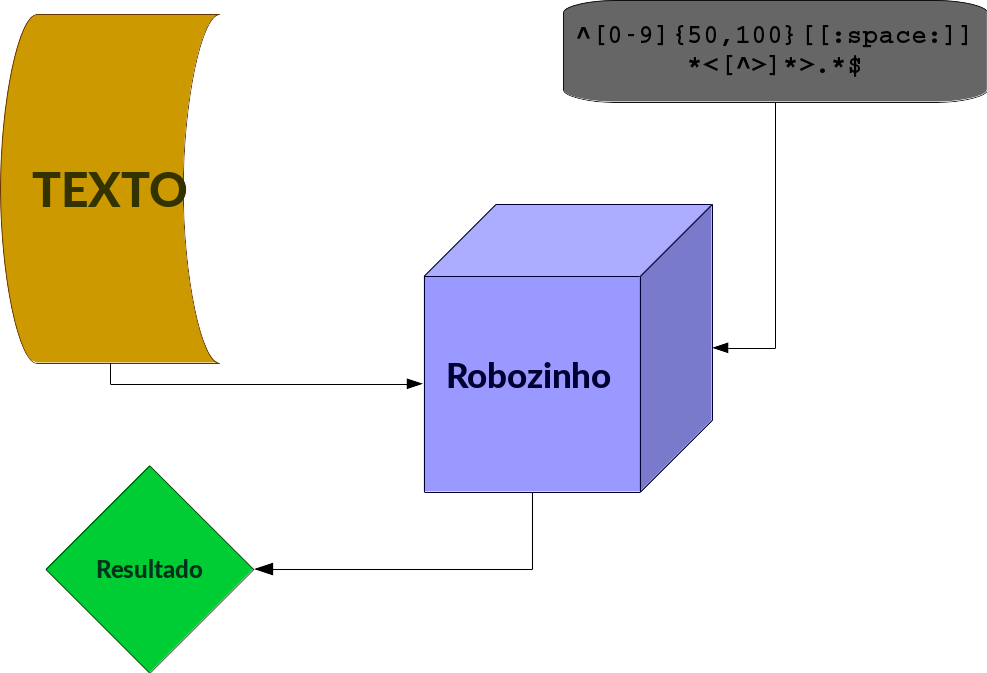
\includegraphics[height=0.75\textheight]{./imagens/re/como-vai-funcionar.png}
\caption{Como vamos abordar as RE}
\end{figure}
\end{frame}

\subsection{Livro}

\begin{frame}
\frametitle{[Expressões Regulares] Uma abordagem divertida}

\begin{figure}[h]
\centering

\includegraphics[height=0.75\textheight]{./imagens/re/piazinho.jpg}
\caption{Essa apresentação foi \azul{inspirada}, \azul{causada} e \azul{é} sobre esse livro.}
\end{figure}
\end{frame}



%-----------------------------------
\newcommand{\meta}[2]{
	\begin{frame}
		\frametitle{#1}
		\centering
		{\fontsize{5cm}{1em}\selectfont \textbf{#2}}
	\end{frame}
}
%-----------------------------------


\section{Metacaracteres}
\frame{\tableofcontents[currentsection]}

\subsection{Caracteres e Metacaracteres}

\begin{frame}
	\frametitle{Você sabe o que são os metacaracteres?}
	
	\begin{itemize}
		\item Se você não conhecia essas belezinhas de \textit{expressões regulares} você só utilizou caracteres literais durante toda sua vida;

		\item Metacaracteres, você, você metacaracteres;

		\item Como isso vai fazer diferença na minha vida?

		\item Diferença dos robozinhos.		
	\end{itemize}
\end{frame}

\begin{frame}
	\begin{figure}
		\centering
			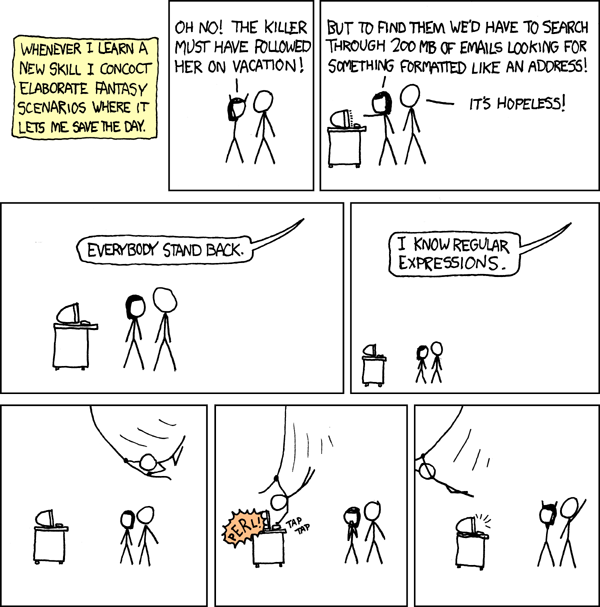
\includegraphics[height=0.8\textheight]{imagens/re/regular_expressions.png}
		\caption{Expressões Regulares salvando o dia}
	\end{figure}

\end{frame}

\begin{frame}
	\frametitle{Tipos}
	\Large{\azul{Representante} e \azul{Quantificador}}
\end{frame}

\subsection{Tipo representante}

%------------------------------------------------
\meta{Ponto}{.}

\begin{frame}
	\frametitle{O ponto}
	\Large{O ponto casa com \azul{TUDO}.}
	
	i.e., o ponto casa com qualquer caractere!

	\azul{Pergunta}: o ponto casa com um ponto?
\end{frame}

\begin{frame}
	\begin{figure}
		\centering
		
\includegraphics[height=0.8\textheight]{./imagens/re/sad_joker.jpeg}
		\caption{O ponto é o coringa solitário.}
	\end{figure}
\end{frame}

\begin{frame}
	\frametitle{Casamento do ponto}
	\begin{center}
		\begin{tabular}{ c | c }
		\textbf{Expressão}	& \textbf{Casa com...}		\\ \hline
		n.o			& nao, não, n40, noo...  	\\ \hline
		.u			& au, bu, du...		 	\\ \hline
		12.45			& 12:45, 12 45, 12.45... 	\\ \hline
		\end{tabular}
	\end{center}

\end{frame}

%------------------------------------------------
\meta{Lista}{[...]}

\begin{frame}
	\frametitle{A lista}
	\begin{itemize}
		\item \Large{A lista casa com \azul{TODOS} os caracteres dentro dela.}
		\item \textbf{Exemplos}: [abc], [123], [letras]...
		\item \large{\bf Dentro da lista todo mundo é LITERAL.}
		\begin{itemize}
			\item O ponto dentro da lista é literal;
		\end{itemize}
	\end{itemize}
\end{frame}

\begin{frame}
	\frametitle{Mentiroso!}
	\begin{itemize}
		\item Lembra que eu falei que todo mundo dentro lista era literal? Então... \Large{\bf EU MENTI \vermelho{MUAHAHAHA}}.
	\end{itemize}
\end{frame}

\begin{frame}
	\frametitle{Mentiroso (nem tanto, vai)!}
	\begin{itemize}
		\item Lembra que eu falei que todo mundo dentro lista era literal? Então...
		\begin{itemize}
			\item Todo caractere que se acha fora da lista, lá dentro não serve pra nada ou tem outro significado;
			\item É como se ela tivesse um mundinho dentro dela, só dela, onde ela dita as regras.
		\end{itemize}
	\end{itemize}
\end{frame}
%------------------------------------------------
\meta{Lista Negada}{[\textasciicircum...]}

\begin{frame}
	\frametitle{A lista negada}
	\begin{itemize}
		\item \Large{A \azul{lista negada} casa com \azul{TODOS} os caracteres que \textbf{\vermelho{NÃO}} estão dentro dela.}
		\item Ou seja, ela não é tão seletiva quanto a lista, tampouco liberal quanto o ponto. Ela sabe com quem não quer casar;
		\item \textbf{Exemplos}: [\textasciicircum abc], [\textasciicircum 123], [\textasciicircum letras]...
	\end{itemize}
\end{frame}

%SOBRE LISTAS--------------------------------------
\begin{frame}
	\frametitle{Intervalos}
	
	\begin{itemize}
		\item Como você faria uma expressão regular para casar com dois números consecutivos?
	\end{itemize}
\end{frame}

\begin{frame}
	\frametitle{Intervalos}
	
	\begin{itemize}
		\item Como você faria uma expressão regular para casar com dois números consecutivos?
		\begin{itemize}
			\item "\textbf{[0123456789][0123456789]}"?
		\end{itemize}
	\end{itemize}
\end{frame}

\begin{frame}
	\frametitle{Intervalos}

	\begin{itemize}
		\item O traço (-) é um operador não literal dentro da lista;
		\item Ele foi criado para representar intervalos:
			\begin{itemize}
				\item \lista{0-9} é igual a \lista{0123456789};
				\item \lista{a-z} é igual a \lista{abcdefghijklmnopqrstuvwxyz};
				\item \lista{A-Z} é igual a \lista{ABCDEFGHIJKLMNOPQRSTUVWXYZ};
				\item \lista{0-9a-zA-Z}
				\item \lista{ -\textasciitilde}
			\end{itemize}
	\end{itemize}
\end{frame}

\begin{frame}
	\frametitle{Intervalos}

	\begin{itemize}
		\item O traço (-) é o único operador não literal dentro da lista;
		\item Ele foi criado para representar intervalos:
			\begin{itemize}
				\item \lista{0-9} é igual a \lista{0123456789};
				\item \lista{a-z} é igual a \lista{abcdefghijklmnopqrstuvwxyz};
				\item \lista{A-Z} é igual a \lista{ABCDEFGHIJKLMNOPQRSTUVWXYZ};
				\item \lista{0-9a-zA-Z};
				\item \lista{ -\textasciitilde}\Huge{\bf \vermelho{???}}
			\end{itemize}
	\end{itemize}
\end{frame}

\begin{frame}
	\frametitle{Exceções}
	
	\begin{itemize}
		\item \textbf{E se eu quiser colocar um traço (-) na lista?}
		\item \textbf{E se eu quiser colocar os colchetes (\lcol  e \rcol) na lista?}
		\item \textbf{E se eu quiser colocar um circunflexo na lista?}
		\item \textbf{E se...}
	\end{itemize}

\end{frame}

\begin{frame}
	\frametitle{Exceções}
	
	\begin{itemize}
		\item \textbf{E se eu quiser colocar um traço (-) na lista?}
		\begin{itemize}
			\item Devemos color o traço no começo ou no final da lista;
			\item \lista{-0-9} $\rightarrow$ Casa com 0 a 9 e traço;
			\item \lista{a-f-} $\rightarrow$ Casa com a a f e traço;
		\end{itemize}
		\item \textbf{E se eu quiser colocar os colchetes (\lcol  e \rcol) na lista?}
		\item \textbf{E se eu quiser colocar um circunflexo na lista?}
		\item \textbf{E se...}
	\end{itemize}

\end{frame}

\begin{frame}
	\frametitle{Exceções}
	
	\begin{itemize}
		\item \textbf{E se eu quiser colocar um traço (-) na lista?}
		\item \textbf{E se eu quiser colocar os colchetes (\lcol  e \rcol) na lista?}
		\begin{itemize}
			\item O "colchete abrir" podemos colocar em qualquer lugar:
			\begin{itemize}
				\item \lista{\lcol0-9};
				\item \lista{0-4\lcol*.ç};
			\end{itemize}
			\item O "colchete de fechar" deve ser o primeiro da lista;
			\begin{itemize}
				\item \lista{\rcol0-9} $\rightarrow$ Casa com 0 a 9 ou com \rcol.
				\item \lista{0-9\rcol} $\rightarrow$ Tá errado.
			\end{itemize}
		\end{itemize}
		\item \textbf{E se eu quiser colocar um circunflexo na lista?}
		\item \textbf{E se...}
	\end{itemize}

\end{frame}

\begin{frame}
	\frametitle{Exceções}
	
	\begin{itemize}
		\item \textbf{E se eu quiser colocar um traço (-) na lista?}
		\item \textbf{E se eu quiser colocar os colchetes (\lcol  e \rcol) na lista?}
		\item \textbf{E se eu quiser colocar um circunflexo na lista?}
			\begin{itemize}
				\item \lista{a-z\textasciicircum}$\rightarrow$casa com caracteres de a a z e \textasciicircum;
				\item \lista{\textasciicircum a-z}$\rightarrow$lista negada: casa com qualquer coisa que não seja de a a z.
			\end{itemize}
		\item \textbf{E se...}
	\end{itemize}

\end{frame}

\begin{frame}
	\frametitle{Exceções}
	
	\begin{itemize}
		\item \textbf{E se eu quiser colocar um traço (-) na lista?}
		\item \textbf{E se eu quiser colocar os colchetes (\lcol  e \rcol) na lista?}
		\item \textbf{E se eu quiser colocar um circunflexo na lista?}
		\item \textbf{E se...}
		\begin{itemize}
			\item Mais alguma coisa/dúvida?
		\end{itemize}
	\end{itemize}

\end{frame}

\begin{frame}
	\frametitle{Casamento das listas}
	\begin{center}
	\begin{tabular}{ c | c }
		\textbf{Expressão} & \textbf{Casa com...} \\ \hline
		n[aãAÃ]o	&	nao, não, nAo, nÃo \\ \hline
		12[:. ]45	&	12:45, 12.45, 12 45 \\ \hline
		funcao.[ch]	&	funcao.c, funcao.h   \\ \hline
		[][-]		&	\textbf{???}		\\ \hline

	\end{tabular}
	\end{center}
\end{frame}

\begin{frame}
	\frametitle{Casamento das listas}
	\begin{center}
	\begin{tabular}{ c | c }
		\textbf{Expressão} & \textbf{Casa com...} \\ \hline
		n[aãAÃ]o	&	nao, não, nAo, nÃo \\ \hline
		12[:. ]45	&	12:45, 12.45, 12 45 \\ \hline
		funcao.[ch]	&	funcao.c, funcao.h   \\ \hline
		[][-]		&	[, ], -		\\ \hline
	\end{tabular}
	\end{center}
\end{frame}

%------------------------------------------------
\subsection{Tipo Quantificador}

%------------------------------------------------
\meta{Opcional}{?}

%------------------------------------------------
\meta{Asterisco}{*}

%------------------------------------------------
\meta{Mais}{+}

%------------------------------------------------
\meta{Chaves}{ \{m,n\} }

%------------------------------------------------
\subsection{Tipo Âncora}

%------------------------------------------------
\meta{Circunflexo}{\textasciicircum}

%------------------------------------------------
\meta{Cifrão}{\$}

%------------------------------------------------
\meta{Borda}{\textbackslash b}

%------------------------------------------------
\subsection{Outros}

%------------------------------------------------
\meta{Ou}{|}

%------------------------------------------------
\meta{Escape}{\textbackslash n}

%------------------------------------------------
\meta{Grupo}{(...)}

%------------------------------------------------
\meta{Retrovisor}{\textbackslash 1...\textbackslash 9}


\section{Exercícios}
\frame{\tableofcontents[currentsection]}

\begin{frame}
\frametitle{Exercícios}
\begin{enumerate}
	\item Baixe um arquivo html de algum site, e extraia com o comando egrep todos os parágrafos entre <p> <\textbackslash p>

	\item Em um código-fonte, encontre todas as funções que retornam inteiros

	\item Abra o arquivo /var/log/kern.log[0-9]? \footnote{Isso é uma expressão regular :)} do seu computador e execute o egrep para achar TODOS os ipv6. i.e., são conjuntos de hexadecimais que vão de 0 a 9, depois de A a F, separados por :. Perceba que o ipv6 pode ser simplificado, zeros seguidos se transformam em ::.

\end{enumerate}
\end{frame}


\section{Aplicações}

\newcommand{\aplicacao}[1]{
	\begin{frame}
		\begin{figure}
			\centering
			\includegraphics[height=0.8\textheight]{./imagens/collage/collage#1.png}
		\end{figure}
	\end{frame}
}

\aplicacao{0}
\aplicacao{1}
\aplicacao{2}


%------------------------------------------------

\section{Referências}

\begin{frame}
\frametitle{Referências}
\bibliography{regex-coders}
\end{frame}

%------------------------------------------------

\section{FIM}
\begin{frame}
\centerline{Dúvidas?}
\titlepage
\end{frame}

%----------------------------------------------------------------------------------------
\end{document}
